\documentclass[11pt]{article}

\usepackage[utf8]{inputenc}
\usepackage[T1]{fontenc}
\usepackage{amsmath,amssymb,amsthm}
\usepackage{hyperref}
\usepackage{graphicx}
\usepackage{geometry}
\geometry{margin=2.5cm}
\usepackage{tikz}
\usepackage{pgfmath}
\usepackage{mathtools}

\newtheorem{theorem}{Theorem}

\theoremstyle{definition}
\newtheorem{definition}{Definition}[section]

\title{Trigonometry without $\pi$: a constructive approach}
\author{Daniel de Rauglaudre (alias roglo)}
\date{\today}

\begin{document}

\maketitle

\begin{abstract}
We present a construction of trigonometry where angles are not real
numbers, but pairs $(x,y)$ such that $x^2 + y^2 = 1$. Several classic
trigonometric formulas naturally emerge during this construction,
which leads to defining the division of an angle by an integer using a
convergent sequence. This construction does not require the prior
definition of the constant $\pi$, which is never used. All results are
formally proven using the Coq proof assistant.
\end{abstract}

\section{Introduction}

... to be done ...

\section{Basic Construction}

In classical trigonometry, angles are real numbers. The set \( A \) of
angles is therefore defined by

\[
A ::= \mathbb{R}
\]

\noindent Here, we set aside this definition and instead define:

\[
A ::= \{ \; (x, y) \; | \; x^2 + y^2 = 1 \; \}
\]

\noindent In other words, an angle is defined by a point on the unit
circle. This point represents the angle between the positive \( x
\)-axis and the line segment from the origin \( O \) to the point.

\

\noindent The angle \( (x, y) \) is illustrated below:

\

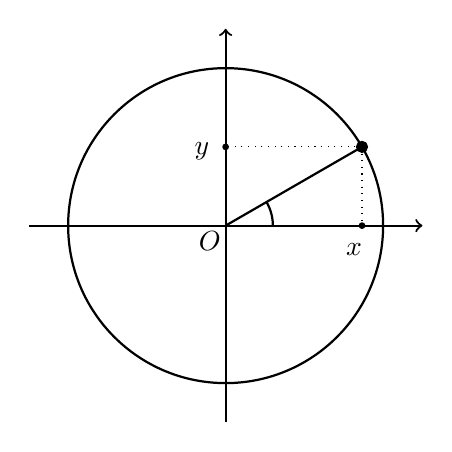
\begin{tikzpicture}
    \draw[thick] (0,0) circle(2);
    \draw[->, thick] (-2.5, 0) -- (2.5, 0);
    \draw[->, thick] (0, -2.5) -- (0, 2.5);
    \node at (-0.2,-0.2) {$O$};

    \pgfmathsetmacro{\px}{cos(30)}
    \pgfmathsetmacro{\py}{sin(30)}
    \coordinate (P) at (\px*2, \py*2);
    \draw[fill] (P) circle (2pt);
    \draw[thick] (0,0) -- (P);
    \draw[thick] (0.6,0) arc[start angle=0, end angle=30, radius=0.6];

    \draw[dotted] (P) -- (\px*2, 0);
    \draw[fill] (\px*2, 0) circle (1pt);
    \node at ({\px*2 - 0.1}, -0.3) {$x$};

    \draw[dotted] (P) -- (0, \py*2);
    \draw[fill] (0, \py*2) circle (1pt);
    \node at (-0.3, {\py*2 - 0.05}) {$y$};
\end{tikzpicture}

\

\

\noindent In our setting, an angle \( \theta \) is not a real number,
but a triple of the form
\[
\theta = (x, y, p),
\]
where \( (x, y) \in \mathbb{R}^2 \), and \( p \) is a proof (or
witness) that \( x^2 + y^2 = 1 \); we define:
\[
\cos(\theta) \coloneqq x, \qquad \sin(\theta) \coloneqq y.
\]

\noindent While in classical mathematics, cosine and sine are defined
by power series, here they are just the first two components of the
triplet. The theorem:
\[
\cos^2(\theta) + \sin^2(\theta) = 1
\]
is true by definition: its proof is $p$, the third component of the
triplet.

\

\noindent In the following, we sometimes represent an angle just as
the pair $(x, y)$, the third component being implicit.

\

\subsubsection*{Drawback}

The difficulty arises from the arithmetic of angles. In classical
trigonometry, this issue does not appear, since angles are treated as
real numbers. Any operation that is defined on the reals—addition,
subtraction, multiplication, inversion, and so on—is directly
applicable to angles.

However, when we think of angles as points on the unit circle, we can
no longer rely on the standard algebraic operations. These points, in
themselves, do not carry any inherent arithmetic structure. In order
to define such operations, we must construct them from scratch. We
begin with addition in the next section.

\section{Addition of angles}

If we have two angles $(x, y, p)$ and $(x', y', p')$, we want to
define an addition, giving a third angle $(x'', y'', p'')$, such that
$x''^2+y''^2=1$.
\[
(x, y, p) + (x', y', p') ::= (x'', y'', p'')
\]

\

\noindent The solution comes from normal trigonometry. If we have two
angles $a$ and $b$, we now that
\[
cos(a+b) = cos\;a\;.\;cos\;b - sin\;a\;.\;sin\;b
\]
\[
sin(a+b) = sin\;a\;.\;cos\;b + cos\;a\;.\;sin\;b
\]

\

\noindent In our trigonometry, if we consider that the angle $(x, y,
p)$ is ``$a$'', and the angle $(x', y', p')$ is ``$b$'', the angle
$(x'', y'', p'')$ is ``$a + b$''. Applying the classical formulas
above, we can define the addition of angles as
\[
(x, y, p) \boldsymbol{+} (x', y', p') \coloneqq (x x' - y y', x y' + y
x', p'').
\]
where $p''$ is the proof that that the sum of the squares of first two
commponents is 1. This is a consequence of $p$ and $p'$. The two
classical formulas above, about $cos(a+b)$ and $sin(a+b)$, are now
true by definition of $+$.

\section{Additive group}

Addition of angles is trivially commutative, and associativity can
also be proven. The neutral element is $(1, 0)$, the null angle. It
says that $cos\;0=1$ and $sin\;0=0$. The inverse element of $(x, y)$
is $(x, -y)$, expressing that $cos\;(- \theta) = cos\;\theta$ and
$sin\;(- \theta) = - sin\;\theta$.

\

\noindent Like for all additive groups, it is possible to define
external multiplication by a natural $n$, by adding the element $n$
times:
\[
  n \; \theta ::=
  \underbrace{\theta + \theta + ... + \theta}_{n \; times}
\]

\

What about {\em multiplication} of two angles? In our framework, it
seems not possible. Because {\em addition} of angles is actually {\em
  multiplication} of complex numbers. Perhaps, then, multiplication of
angles could be something that {\em exponentiation} of complex
numbers? But this intuition seems not to work.

Moreover, as far as geometry is concerned, multiplication of angles
seems to have no meaning. In this work, we didn't define it.

This has a consequence: it is not possible to define exponentiation of
imaginary angles either, which we found in the famous expression
$e^{i\theta}$ of classical trigonometry, supposed to be equal to
$cos\;\theta+i\;sin\;\theta$ (Euler's formula), because exponentiation
is defined by a power series holding powers of its parameter:
\[
e^x = \sum_{n=0}^\infty{\; \frac{x^n}{n!}}
\]

i.e. its parameter $x$ {\em multiplied} several times by itself. Since
multiplication of angles doesn't exist, Euler's formula doesn't work,
but we see further, that de Moivre's formula works in our trigonometry
and we use it. Remainder: de Moivre's formula is:
\[
(cos \; \theta + i \; sin \; \theta)^n = cos (n \theta) + i \; sin (n
\theta)
\]

\

\noindent But what we need, for the moment, is division by a
natural. We defined above multiplication by a natural. Division is
more complicated but we see in next sections that it is possible to
define it.

\section{Trying to define the division of an angle by a natural}

...

\section{Conclusion}

... to be done ...

\paragraph{Code source :}
\url{https://github.com/roglo/coq_sensitivity/tree/master/trigo_without_pi}

\end{document}
